\chapter{Теоретические сведения о визуализации графов}
Визуализация графа — это графическое представление вершин и ребер графа. 
Визуализация строится на основе исходного графа, но направлена на получение дополнительных атрибутов вершин и ребер: размера, цвета, 
координат вершин, толщины и геометрии ребер. Помимо этого, в задачи визуализации входит определение масштаба представления визуализации. 
Для различных по своей природе графов, могут быть более применимы различные варианты визуализации. 
Таким образом задачи, входящие в последовательность подготовки графа к визуализации, формулируются исходя из эстетических и эвристических критериев.

\section{Алгоритмы раскладки графов}

Раскладка неориентированных графов испольуется при проектировании топологии СБИС, 
целью которого является оптимизация схемы для получения наименьшего количества пересечений линий. 

Пружинная система запускается со случайным начальным состоянием, и вершины соответственно перемещаются под действием пружинных сил. 
Оптимальная компоновка достигается за счет того, что энергия системы сводится к минимуму.

\subsection{The Spring Model}
Модель spring-embedder была первоначально предложена Eades (1984) и в настоящее время является одним из самых популярных алгоритмов 
для рисования неориентированных графов с прямолинейными ребрами, широко используемого в системах визуализации информации.

Алгоритм Идеса следует двум эстетическим критериям: равномерная длина ребер и максимально возможная симметрия. 
В модели Spring-Embedder вершины графа обозначаются набором колец, и каждая пара колец соединена пружиной. 
Пружина связана с двумя видами сил: силами притяжения и силами отталкивания, в зависимости от расстояния и свойств соединительного пространства.

\subsection{Local Minimum}
Модель spring-embedder привела к созданию ряда модифицированных и расширенных алгоритмов раскладки неориентированных графов. 
Например, силы отталкивания обычно вычисляются между всеми парами вершин, а силы притяжения могут быть рассчитаны только между 
соседними вершинами. Упрощенная модель уменьшает временную сложность: вычисление сил притяжения между соседями выполняется за O(|E|), 
хотя вычисление силы отталкивания выполняется за O(|V|²), что в является недостатком алгоритмов с n телами. Камада и Каваи (1989) представили 
алгоритм, основанный на модели пружинного внедрения Идса, который пытается достичь следующих двух критериев или эвристик рисования графа: 
количество пересечений ребер должно быть минимальным, а вершины и ребра распределены равномерно. 

Цель алгоритма состоит в том, чтобы найти локальный минимум энергии в соответствии с вектором градиента $\sigma = 0$, что является необходимым, 
но не достаточным условием глобального минимума энергии. С точки зрения вычислительной сложности, такой поиск требует большого количества 
операций, поэтому в реализацию часто включаются дополнительные элементы управления, чтобы гарантировать, что пружинная система не 
окажется в локальном минимуме. В отличие от алгоритма Идеса, который явно не включает закон Гука, алгоритм Камады и Каваи перемещает 
вершины в новые положения по одной, так что общая энергия пружинной системы уменьшается с новой конфигурацией. Он также вводит понятие желаемого 
расстояния между вершинами на визуализации: расстояние между двумя вершинами пропорционально длине кратчайшего пути между ними.

\subsection{Force-Directed Placement}
Алгоритм Фрухтермана-Рейнгольда основан на модели пружинного встраивания Идса. Он равномерно распределяет узлы, минимизируя пересечения ребер, 
а также поддерживает одинаковую длину ребер. В отличие от алгоритма Камада-Каваи, алгоритм Фрухтермана-Рейнгольда использует две 
силы (силы притяжения и силы отталкивания) для обновления узлов, а не использует функцию энергии с теоретическим графическим расстоянием.

Алгоритм Фрухтермана-Рейнгольда выполняется итеративно, и все узлы перемещаются одновременно после расчета сил для каждой итерации. 
Алгоритм добавляет атрибут «смещения» для контроля смещения положения узлов. В начале итерации алгоритм Фрухтермана-Рейнгольда вычисляет 
начальное значение смещения для всех узлов с использованием силы отталкивания (fr). Алгоритм также использует силу притяжения (fa) для 
многократного обновления визуального положения узлов на каждом ребре. Наконец, он обновляет смещение положения узлов, используя значение смещения.

\chapter{Выполнение практикума}

Мой вариант №6, поэтому визуализировались данные из необходимого файла №6.

Для визуализации графа был использован код примера с модификацией в файле исходных текстов было реализовано простое чтение текстовых файлов для удобной загрузке большого количества вершин и связей между ними напрямую из файла;
\begin{lstlisting}[label=host, caption={Модификация файла host\_main.cpp}]
 unsigned int* host2gpc_ext_buffer[LNH_GROUPS_COUNT][LNH_MAX_CORES_IN_GROUP];
unsigned int messages_count = 0;
unsigned int u, v, w;

__foreach_core(group, core)
{
	host2gpc_ext_buffer[group][core] = (unsigned int*)lnh_inst.gpc[group][core]->external_memory_create_buffer(16 * 1048576 * sizeof(int)); //2*3*sizeof(int)*edge_count);
	offs = 0;
	
	std::ifstream file(argv[3], std::ios::in);
	
	if (!file.is_open())
	{
		std::cout << "Cannot open input file." << std::endl;
		
		return EXIT_FAILURE;
	}
	
	for (std::string line; std::getline(file, line); )
	{
		std::vector<std::string> tokens = split(line, '\t');
		
		if (tokens.size() != 2)
		{
			for (auto token : tokens)
			std::cout << token << " ";
			std::cout << std::endl;
			std::cout << "Incorrect tokens count in file: expected 3, got " << tokens.size() << "." << std::endl;
			
			return EXIT_FAILURE;
		}
		
		u = std::stoul(tokens[0]);
		v = std::stoul(tokens[1]);
		w = 1;
		
		//Граф должен быть связным
		EDGE(u, v, w);
		EDGE(v, u, w);
		messages_count += 2;
	}
	
	lnh_inst.gpc[group][core]->external_memory_sync_to_device(0, 3 * sizeof(unsigned int) * messages_count);
}
\end{lstlisting}
Полученные изображения графа в box-раскладке и force-раскладке приведены на рисунках 2.1 -- 2.2.
\begin{figure}[H]
	\centering
	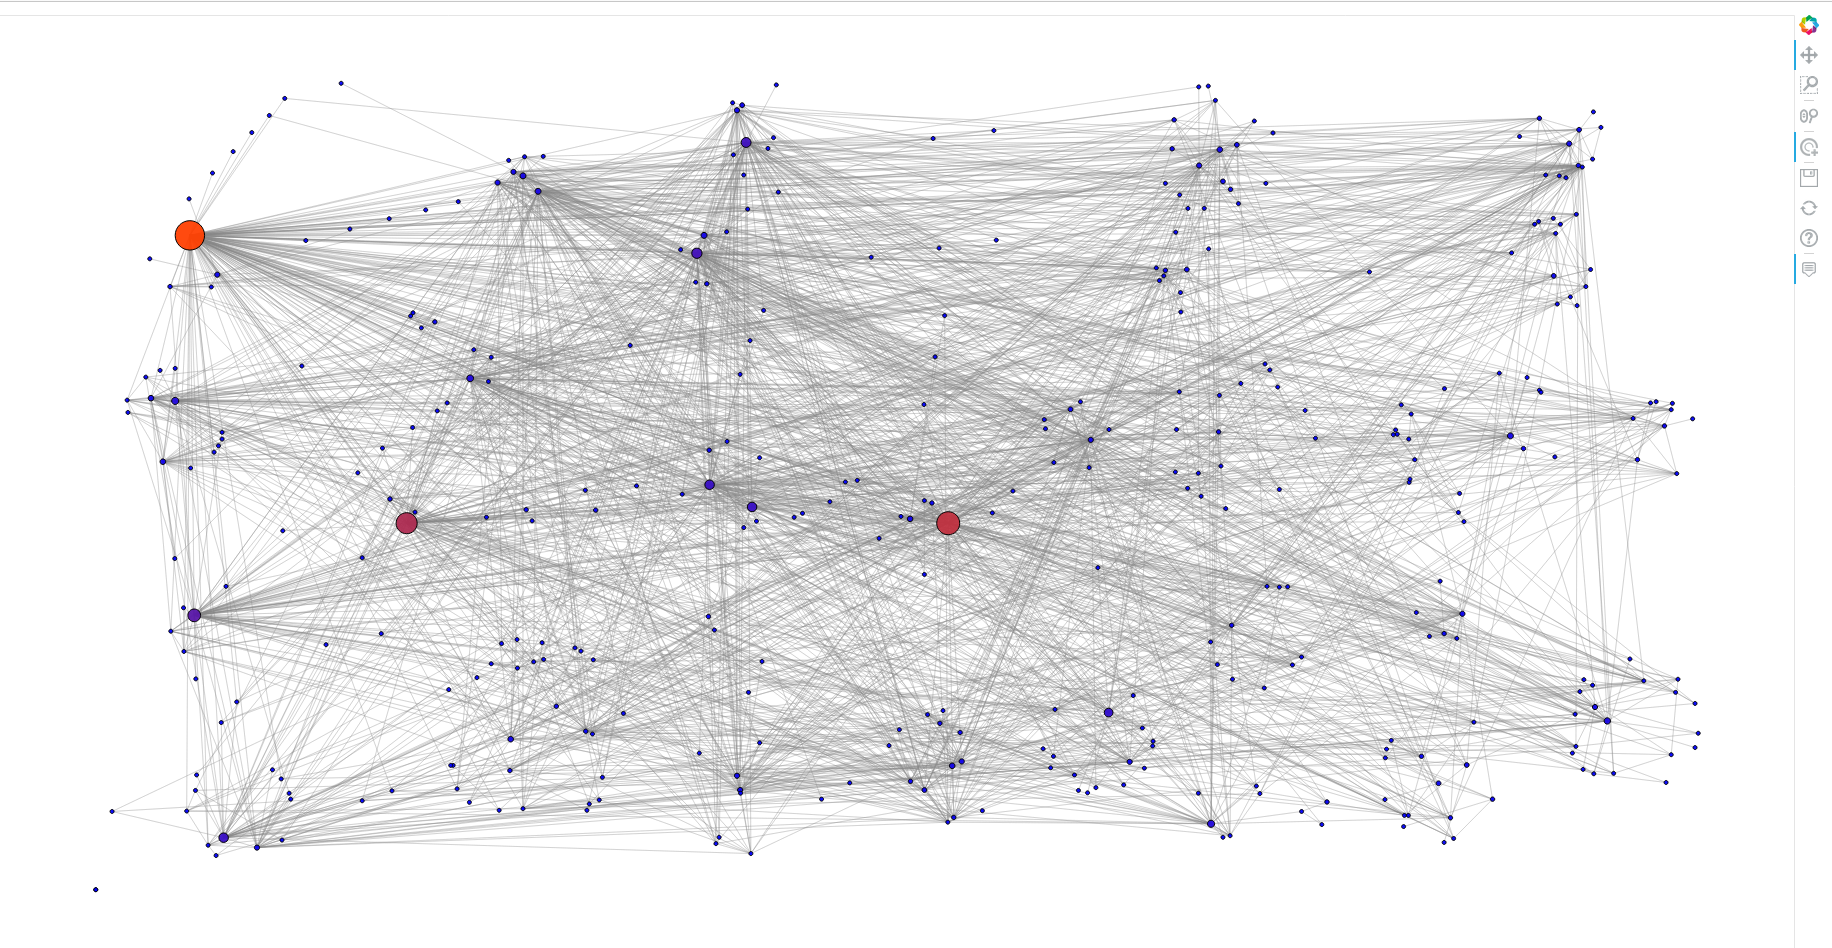
\includegraphics[width=1\linewidth]{box}
	\caption{}
	\label{fig:box}
\end{figure}

\begin{figure}[H]
	\centering
	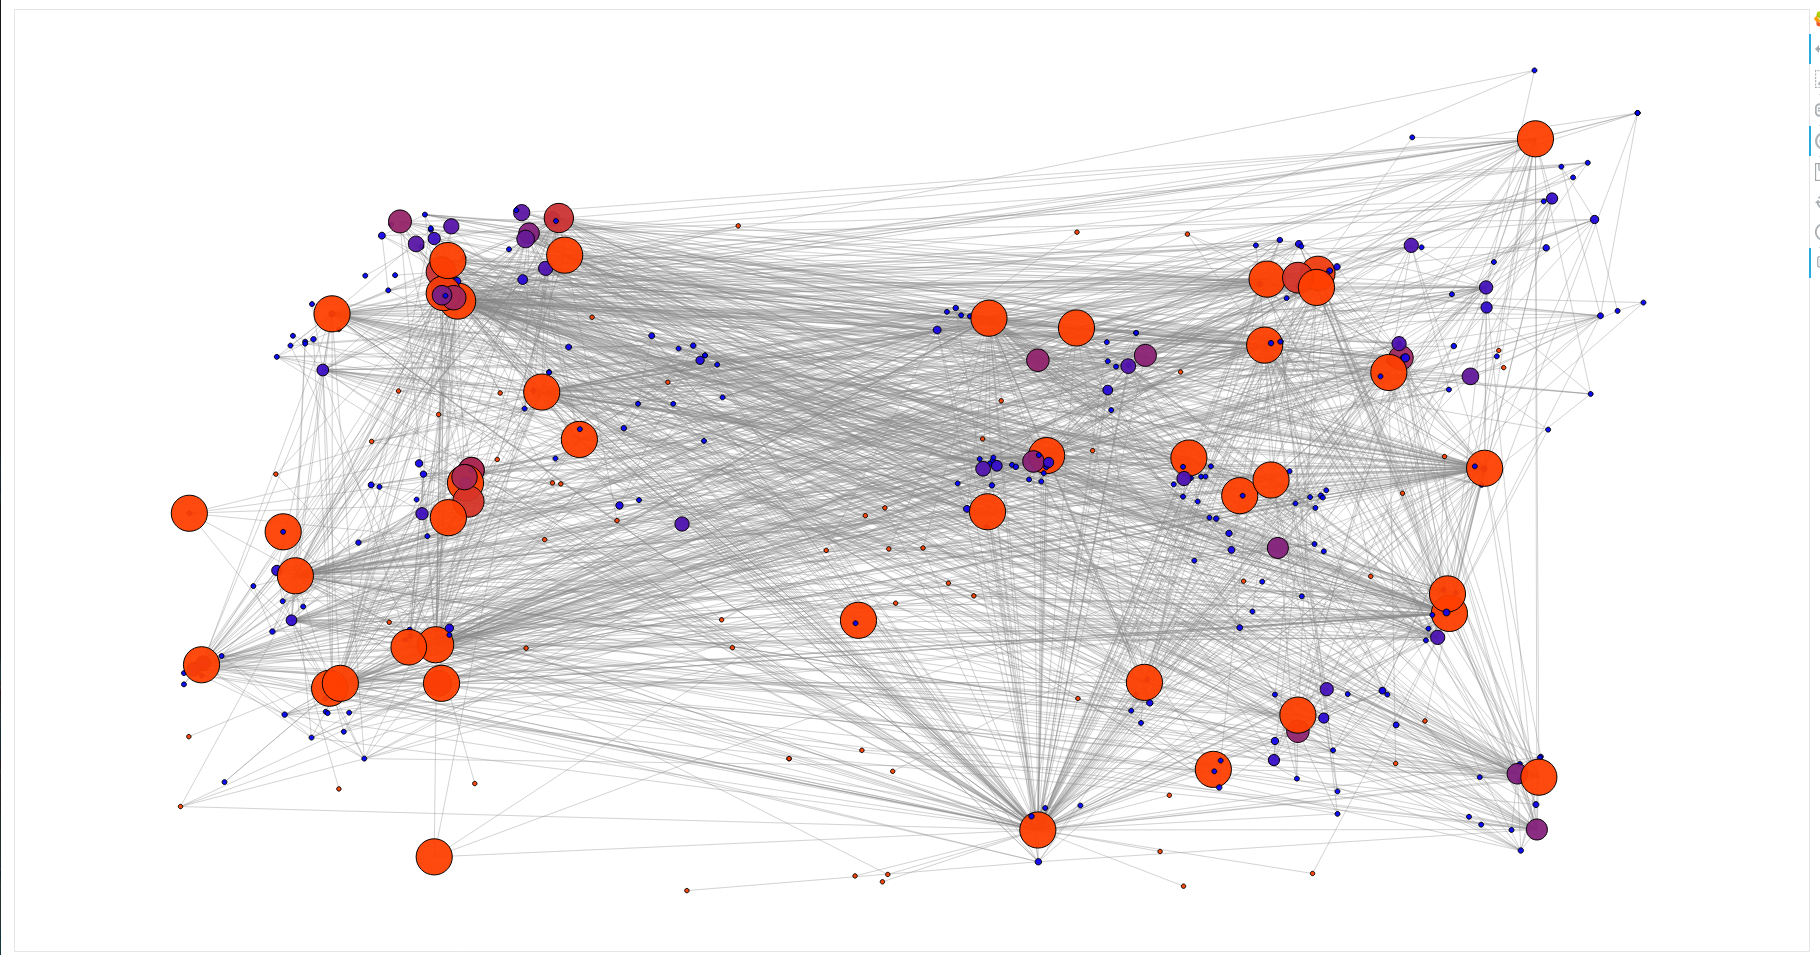
\includegraphics[width=1\linewidth]{force}
	\caption{}
	\label{fig:force}
\end{figure}

